\appendix
\chapter{Graph Analysis}
\label{app:graphs}

\section{MRN114}
\begin{figure}[h!]
\centering
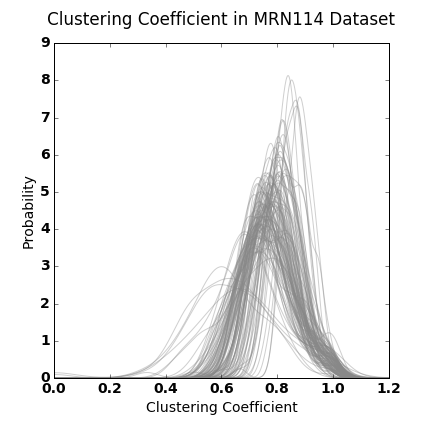
\includegraphics[width=0.4\textwidth]{./stats/MRN114-cc.png}
\end{figure}

\begin{figure}[h!]
\centering
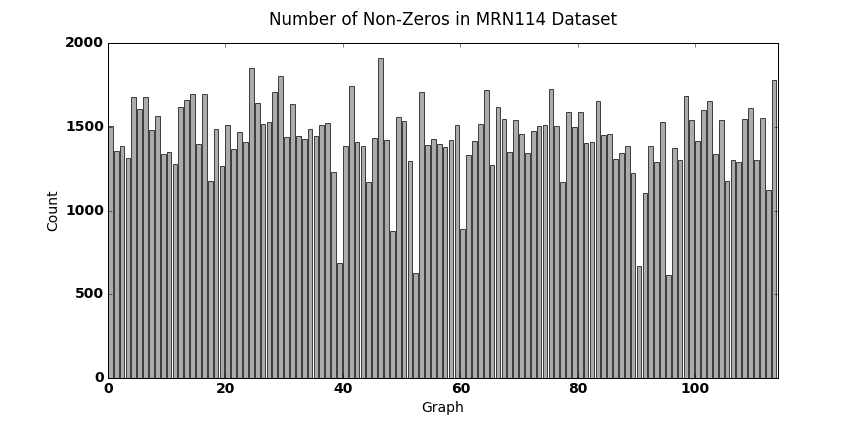
\includegraphics[width=0.8\textwidth]{./stats/MRN114-nnz.png}
\end{figure}

\begin{figure}[h!]
\centering
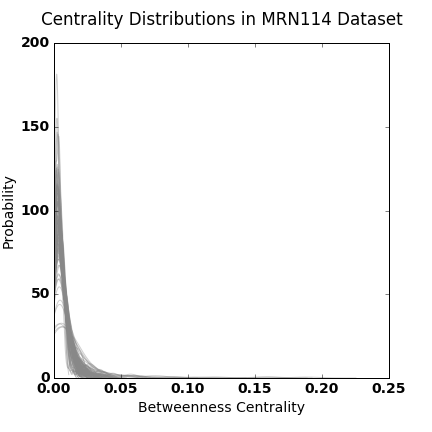
\includegraphics[width=0.4\textwidth]{./stats/MRN114-centrality.png}
\end{figure}

\begin{figure}[h!]
\centering
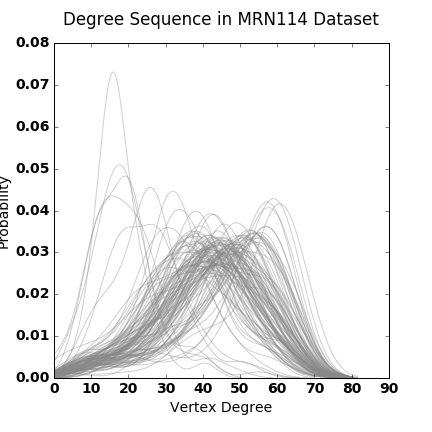
\includegraphics[width=0.4\textwidth]{./stats/MRN114-degree.png}
\end{figure}

\begin{figure}[h!]
\centering
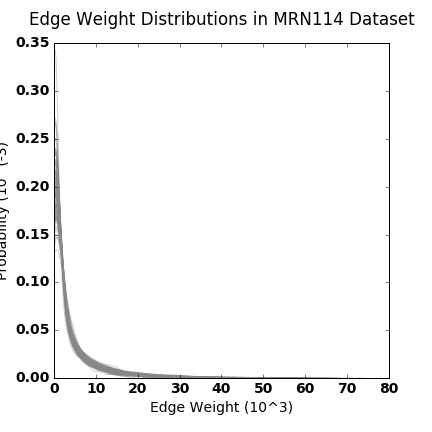
\includegraphics[width=0.4\textwidth]{./stats/MRN114-edgeweight.png}
\end{figure}

\clearpage
\section{SWU4}
\begin{figure}[h!]
\centering
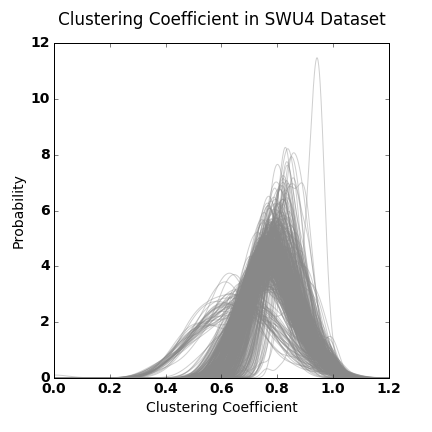
\includegraphics[width=0.4\textwidth]{./stats/SWU4-cc.png}
\end{figure}

\begin{figure}[h!]
\centering
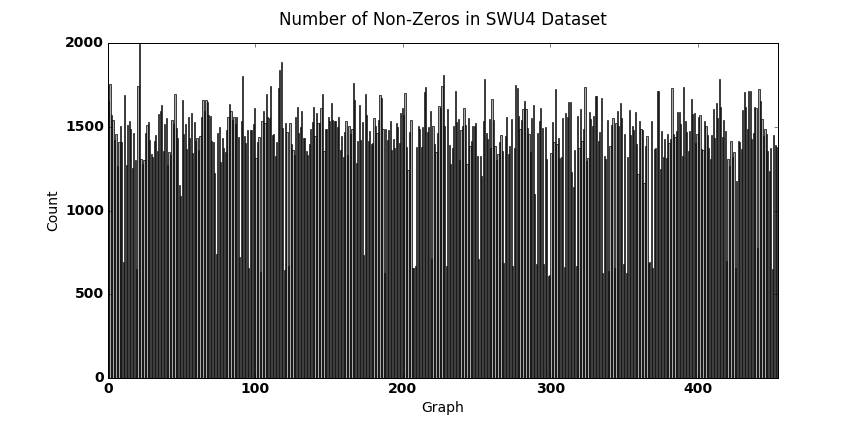
\includegraphics[width=0.8\textwidth]{./stats/SWU4-nnz.png}
\end{figure}

\begin{figure}[h!]
\centering
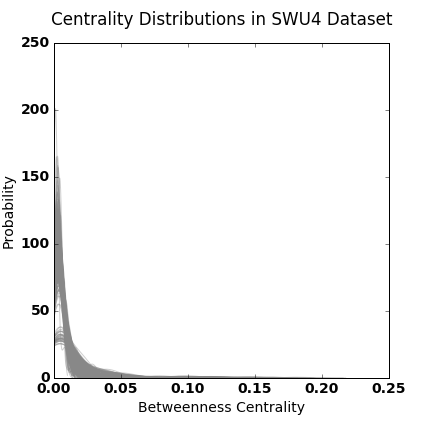
\includegraphics[width=0.4\textwidth]{./stats/SWU4-centrality.png}
\end{figure}

\begin{figure}[h!]
\centering
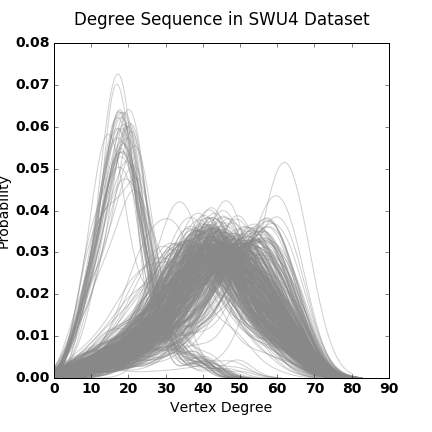
\includegraphics[width=0.4\textwidth]{./stats/SWU4-degree.png}
\end{figure}

\begin{figure}[h!]
\centering
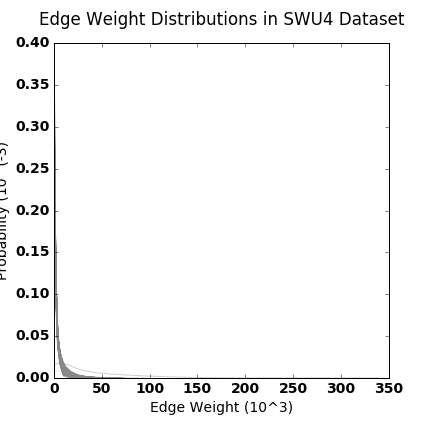
\includegraphics[width=0.4\textwidth]{./stats/SWU4-edgeweight.png}
\end{figure}
